%%%%%%%%%%%%%%%%%%%%%%%%%%%%%%%%%%%%%%%%%%%%%%%%%%%%%%%%%%%%%%%%%%
%%%%%%%% ICML 2017 EXAMPLE LATEX SUBMISSION FILE %%%%%%%%%%%%%%%%%
%%%%%%%%%%%%%%%%%%%%%%%%%%%%%%%%%%%%%%%%%%%%%%%%%%%%%%%%%%%%%%%%%%

% Use the following line _only_ if you're still using LaTeX 2.09.
%\documentstyle[icml2017,epsf,natbib]{article}
% If you rely on Latex2e packages, like most moden people use this:
\documentclass{article}

% use Times
\usepackage{times}
% For figures
\usepackage{graphicx} % more modern
%\usepackage{epsfig} % less modern
%\usepackage{subfigure} 
\usepackage{caption}
\usepackage{subcaption}

% For citations
\usepackage{natbib}

% AMS stuff
\usepackage{amsmath, amsthm, amssymb}
\usepackage{dsfont}
\newtheorem{theorem}{Theorem}
\newtheorem{lemma}{Lemma}
\newtheorem{cor}{Corollary}

% For algorithms
\usepackage{algorithm}
\usepackage{algorithmic}

% As of 2011, we use the hyperref package to produce hyperlinks in the
% resulting PDF.  If this breaks your system, please commend out the
% following usepackage line and replace \usepackage{icml2017} with
% \usepackage[nohyperref]{icml2017} above.
\usepackage{hyperref}
\usepackage{booktabs}


% Packages hyperref and algorithmic misbehave sometimes.  We can fix
% this with the following command.
\newcommand{\theHalgorithm}{\arabic{algorithm}}

\DeclareMathOperator*{\argmin}{arg\,min}
\DeclareMathOperator*{\argmax}{arg\,max}
% Employ the following version of the ``usepackage'' statement for
% submitting the draft version of the paper for review.  This will set
% the note in the first column to ``Under review.  Do not distribute.''
\usepackage{icml2017} 

% Employ this version of the ``usepackage'' statement after the paper has
% been accepted, when creating the final version.  This will set the
% note in the first column to ``Proceedings of the...''
%\usepackage[accepted]{icml2017}


% The \icmltitle you define below is probably too long as a header.
% Therefore, a short form for the running title is supplied here:
\icmltitlerunning{ Active Learning for CNNs}

\begin{document} 

\twocolumn[
\icmltitle{ Active Learning for Convolutional Neural Networks}

% It is OKAY to include author information, even for blind
% submissions: the style file will automatically remove it for you
% unless you've provided the [accepted] option to the icml2017
% package.

% list of affiliations. the first argument should be a (short)
% identifier you will use later to specify author affiliations
% Academic affiliations should list Department, University, City, Region, Country
% Industry affiliations should list Company, City, Region, Country

% you can specify symbols, otherwise they are numbered in order
% ideally, you should not use this facility. affiliations will be numbered
% in order of appearance and this is the preferred way.

\begin{icmlauthorlist}
\icmlauthor{Ozan Sener}{to}
\icmlauthor{Silvio Savarese}{to}
\end{icmlauthorlist}

\icmlaffiliation{to}{Department of Computer Science, Stanford University, CA, US}

\icmlcorrespondingauthor{Ozan Sener}{ozan@cs.stanford.edu}

% You may provide any keywords that you 
% find helpful for describing your paper; these are used to populate 
% the "keywords" metadata in the PDF but will not be shown in the document
\icmlkeywords{boring formatting information, machine learning, ICML}

\vskip 0.3in
]

% this must go after the closing bracket ] following \twocolumn[ ...

% This command actually creates the footnote in the first column
% listing the affiliations and the copyright notice.
% The command takes one argument, which is text to display at the start of the footnote.
% The \icmlEqualContribution command is standard text for equal contribution.
% Remove it (just {}) if you do not need this facility.

%\printAffiliationsAndNotice{}  % leave blank if no need to mention equal contribution
\printAffiliationsAndNotice{} % otherwise use the standard text.
%\footnotetext{hi}

\begin{abstract} 
Convolutional neural networks(CNNs) have been successfully applied to many recognition and learning task using a universal recipe; very large data-set of supervised examples and a deep layered model. However, this approach is rather restrictive in practice since collecting a large labelled data-set of images is very expensive. One way to ease this problem is coming up with smart ways to query labels among very large dataset of unlabelled images (ie. active learning)%The field of active learning study this problem; however, existing approaches are not effective for CNNs.

In this paper; we first show that existing active learning heuristics are not effective for CNNs even in an oracle case. Our counterintuitive empirical results make us question these heuristics, and inspires us to come-up with a simple but effective method; trying to choose set of queries such that they cover the set of unlabelled images as close as possible. We further present a theoretical justification for this heuristic by presenting a geometric bound over the generalization error of CNNs. Our experiments show that the proposed method significantly outperforms existing approaches in image classification experiments with a large-margin.
\end{abstract} 

\section{Introduction}
Deep convolutional neural networks(CNNs) have shown unprecedented success in many areas of active research in computer vision like image classification, object detection and scene segmentation. Although CNNs are universally successful in many computer vision tasks, they have a major drawback; they need very large amount of labelled data in order to be able to learn their millions of parameters. More importantly, it is almost always better to have more data since accuracy of CNNs typically are never saturated with respect to the dataset size. Hence, there is a constant desire to collect more and more data. Although this behavior is rather desired from an algorithmic perspective (higher representative power is typically better), labelling a dataset is time consuming and an expensive task. These practical considerations bring a critical question; \emph{``what is the optimal way to choose data points to label such that most of the accuracy increase can be obtained given a fixed labelling budget.''}  

The goal of active learning is finding effective ways to choose data points among set of unlabelled data points in order to maximize the accuracy. Although it is not possible to obtain a universally good query strategy \cite{dasgupta}, there exist many heuristics~\cite{settles2010active} to choose set of points to query to a labeler. Although many of these heuristics are effective and perform better than random sampling, they are typically not effective for CNNs. The prevalent belief for this behavior is the fact that CNNs make very confident mistakes. In other words, it is not possible to deduce that a CNN is uncertain and need more data by only looking at its outputs. Although we agree with this observation, our empirical analysis suggests that this is not the main reason behind the ineffectiveness of active learning for CNNs. 

We approach to the problem of active learning purely from geometric approach; and, hypothesis that given a large unlabelled dataset, a desired property of set of points which are labelled is covering this space as efficiently as possible. In other words, we seek set of points to label such that when they are labelled, every unlabelled point in the dataset will have a close labelled neighbor. We formulate this space-covering property in terms of a discrete optimization problem and present an efficient solution. 

We cary out an in-depth analysis of our algorithm both theoretically and empirically. We study the generalization error of CNNs in a very realistic setting and present a bound on the difference between the expected risk and the empirical risk. We further consider the active learning case and present a bound over the risk of the unlabelled data points in terms of distance between unlabelled points and their labelled nearest neighbors. We further study the behavior of our proposed algorithm empirically for the problem of image classification using the CIFAR\cite{cifar} dataset. Our empirical analysis demonstrates a state-of-the-art performance with a large margin. 

\section{Related Work}
There are many areas of active research related to our work. We divide them in the following categories and discuss them separately. 

\noindent\textbf{Active Learning}
Active learning has been widely studies and most of the early work can be found in the classical survey \cite{settles2010active}. It discusses most query strategies like information theoretical methods \cite{mackay1992information} and ensemble approaches \cite{mccallumzy1998employing, freund1997selective}. We will try to review the literature coming after \cite{settles2010active}. 

Bayesian active learning methods typically use a non-parametric model like Gaussian process to estimate the expected improvement of each label \cite{kapoor2007active} or expected error after labels \cite{roy2001toward}. These approaches are typically not applicable to deep learning scenarios since they do not scale to large-scale datasets. Ensemble methods are also not applicable to deep learning because of large parameter space of neural networks. Such ensemble methods requires intractable number of networks to be trained to be effective in a very large dimensional parameter space.

One important class is uncertainty based selection \cite{tong2001support,lewissequential,joshi2009multi,li2013adaptive} which tries to find hard-negatives using heuristics like highest entropy \cite{joshi2009multi}, or geometric distance to decision boundaries \cite{tong2001support,brinker2003incorporating}. We present an empirical result in Section~\ref{neg_res} which motivated us to move away from such techniques. We show that even in the oracle case, such algorithms have very limited accuracy improvement. Indeed, we even observed a drop in the accuracy for the case of semi-supervision when oracle uncertainty is used. 

More recently, we have seen optimization based approaches which can trade-off uncertainty and diversity in order to obtain diverse set of high likely hard-negatives. Elhamifar~et al.  \cite{elhamifar2013convex} design a discrete optimization problem for this purpose and uses its convex surrogate. However, the algorithm uses $n^2$ variables where $n$ is the number of data points. Hence, it does not scale to deep learning case. There are also many discrete optimization based active learning algorithms designed for specific class of machine learning algorithms like k-nearest neighbors and naive Bayes \cite{wei2015submodularity}. Even in algorithm agnostic case, one can design a set-cover algorithm to efficiently cover the hyphotesis space using sub-modularity \cite{guillory2010interactive, golovin2011adaptive}. Our algorithm can be considered in this class; however, we do not use the uncertainty information due to the empirical result we present in the Section~\ref{sec:whatif}. Our algorithm is also the first one which is applied to deep learning and/or convolutional neural networks.

Recently, a discrete optimization based algorithm \cite{BerlindU15} similar to us with strong theoretical guarantees has been presented for k-nearest neighbors(k-NN) type of algorithms in domain shift setting. Although our theoretical analysis borrows many techniques from \cite{BerlindU15}, their results are only valid for k-NN and not applicable to convolutional neural networks. 

To the best-of-our-knowledge, only active learning algorithm designed for deep learning is the framework presented in \cite{wang2016cost}. It is a heuristic based transductive algorithm which assign labels to data-points having high-confidence directly and query labels for the ones having low confidence. We discuss the limitations of \cite{wang2016cost} in detail in Section~\ref{sec:exp}.


\noindent\textbf{Subset Selection}
Closest literature to our work is the problem of subset selection. The subset selection problem considers a dataset and try to choose a subset of it such that the resulting model will perform as close to the model trained on the entire dataset as possible. Formally, this problem can be described as finding a core-set for a dataset such that a model learned over the subset will perform very close to a model learned over the entire dataset. For specific learning algorithms, there are methods like core-sets for SVM \cite{tsang2005core} and core-sets for k-Means and k-Medians \cite{har2005smaller}. However, there is no such method for CNNs.

Most similar to our algorithm is unsupervised subset selection described in \cite{wei2013using}. It uses a facility location in order to find a diverse subset covering the space. Our algorithmic difference is using a slightly different formulation of facility location problem. Instead of the min-sum, we use minimax \cite{facility} form of the facility location. More importantly, we apply this algorithm the first time to the problem of active learning, we also analyze this algorithm in detail both empirically and theoretically for the problem of active learning with CNNs.

 
\noindent\textbf{Semi-Supervised Deep Learning}
Our paper is also related to semi-supervised deep learning since we experiment the active learning both in fully-supervised and semi-supervised scheme. 
One of the early semi-supervised convolutional neural network algorithms was Ladder networks \cite{ladder}. Recently, we have seen adversarial methods which can learn a data-distribution as a result of a two-player non-cooperative game \cite{salimans2016improved,gan_original,dcgan}. These methods are further extended to feature learning by \cite{ali, bigan}. Thanks to the defined two-player game, these methods can perform semi-supervised learning very naturally. We use Ladder networks in our experiments since adversarial architectures are notoriously hard to train. Our algorithm is agnostic to used semi-supervised learning algorithm and can readily be used in any semi-supervised or supervised setting.

\section{Problem Definition}
In this section, we formally define the problem of active learning by setting-up the notation for rest of the paper. We are interested in $C$ class classification problem defined over a compact space $\mathcal{X}$ and a label space  $\mathcal{Y}=\{1,\ldots,C\}$. We also consider a loss function $l(\cdot,\cdot;\mathbf{w}):\mathcal{X}\times \mathcal{Y} \rightarrow \mathcal{R}$ parametrized over the hyphotesis class ($\mathbf{w}$), e.g.\ parameters of the deep learning algorithm. We also assume class-specific regression functions $\eta_c(\mathbf{x})=p(y=c|\mathbf{x})$ to be \mbox{$\lambda^\eta$-Lipschitz} continuous for each $c$.

We consider a large collection of data points which are sampled iid over the space  $\mathcal{Z}=\mathcal{X}\times\mathcal{Y}$ as \mbox{$\{\mathbf{x}_i,y_i\}_{i \in [n]} \sim p_\mathcal{Z}$}. We further consider an initial pool of data-points chosen iid among them as \mbox{$\mathbf{s}^0=\{s^0(j) \in [n]\}_{j \in [m]}$}. 

In our setting, an active learning algorithm has only access to $\{\mathbf{x}_i\}_{i \in [n]}$ and $\{y_{s(j)}\}_{j \in [m] }$. In other words, it can not see the labels of all data points except the initial sub-sampled pool. It is also given a budget $b$ of queries to ask to an oracle and a (semi)supervised learning algorithm $A_{\mathbf{s}}$ which outputs a set of parameters $\mathbf{w}$ given a labelled set $\mathbf{s}$. The active learning with a pool problem can simply be defined as
\begin{equation}
\min_{\mathbf{s}^1 : |\mathbf{s}^1| \leq b} E_{\mathbf{x},y \sim p_\mathcal{Z}} [l(\mathbf{x},y; A_{\mathbf{s}^0 \cup \mathbf{s}^1})]
\end{equation}
In other words, an active learning algorithm can choose $b$ extra points and get it labelled by an oracle to minimize the future expected loss.

There are a few differences between our formulation and the classical definition of active learning. Classical methods consider the case the budget is 1 as $b=1$ but a single point has negligible effect in a deep learning regime. It is also very common to consider multiple round of this game as;
\begin{equation}
\min_{\mathbf{s}^{k+1} : |\mathbf{s}^{k+1}| \leq b} E_{\mathbf{x},y \sim p_\mathcal{Z}} [l(\mathbf{x},y; A_{\mathbf{s}^{0} \cup \ldots, \mathbf{s}^{k+1}})]
\end{equation}
Although it is more realistic, analysis is typically trickier in such a setting. Hence, we consider the greedy version and try to solve the single round of labelling. In practice, we use multiple rounds by solving each single round. We also consider a semi-supervised algorithm instead of a supervised one. Although, the query methods are typically equally applicable in both cases, we empirically observed different behavior.

\section{Active Learning as a Set Cover}
In non-Bayesian setting, active learning problem is typically considered as refining decision boundaries by querying hard-negatives. Hence, using uncertainty is an empirically proven heuristic. However, this heuristic has very limited success in CNNs. This is widely attributed to the fact that the CNNs typically makes very confident mistakes and the confidence values computed via soft-max outputs do not correspond to actual confidence scores. Although we agree with this observation, we further asked the question \emph{would classical query methods work for CNNs if they had accurate uncertainty estimates?}. Although common sense answer is yes, our empirical analysis shows this is typically not the case. We describe this experiment in detail in Section~\ref{sec:whatif}.

Empirical observation of ineffectiveness of uncertainty based approaches, inspired us to design a rather contradictory method for active learning for CNNs. We propose to not use class estimates and/or labels of already labelled data points, instead attack the problem from purely a geometric approach. We design an algorithm based on the heuristic of covering the set of unlabelled data points as efficiently as possible. We explain this algorithm in detail in Section~\ref{sec:alg} and further analyze it empirically in Section~\ref{sec:exp} and theoretically in Section~\ref{sec:analysis}.

\subsection{Ineffectiveness of Uncertainty based Methods in CNNs}
\label{sec:whatif}
It is very common to attribute the ineffectiveness of uncertainty methods in CNNs to the fact that uncertainty estimates based on soft-max outputs are typically not accurate. Hence, it is very common to hypothesize the following using ineffectiveness of uncertainty based methods as a base:

\noindent\textbf{Hypothesis:} \emph{Deep learning algorithms results in an inaccurate estimate of uncertainty hence the uncertainty based methods fail.}

Although this hypothesis is very intuitive considering the many confident mistakes CNNs typically make, it is also very easy to experiment. We simply ask the following question;

\noindent\textbf{Question:} \emph{If CNNs had an accurate estimate of uncertainty, would uncertainty based active learning methods work ?}

This is very easy to experiment by simply replacing the uncertainty estimates in active learning with oracle ground truth loss. In other words, we replace the uncertainty with $l(\mathbf{x}_i,y_i,A_{\mathbf{s}^0})$ for all unlabelled examples $\mathbf{x}_i$. Since, this simply is the oracle for the estimation of the uncertainty, in practice the uncertainty based methods expected to be upper bounded by this oracle. We sample the queries from the normalized form of this function as probability of choosing the $i^{th}$ point as query is $p_i=\frac{l(\mathbf{x}_i,y_i,A_{\mathbf{s}^0})}{\sum_j l(\mathbf{x}_j,y_j,A_{\mathbf{s}^0})}$. We use two loss functions; classification accuracy \mbox{$\mathds{1}[i_i = \argmax_c CNN_c(\mathbf{x}_i;A_{\mathbf{s}^0})]$} and cross entropy
\mbox{$ - CNN_{y_i}(\mathbf{x}_i;A_{\mathbf{s}^0}) -\sum_{c \in [C] \setminus y_i} \log(1-  CNN_{c}(\mathbf{x}_i;A_{\mathbf{s}^0}))$} where $\mathds{1}[\cdot]$ is the indicator function and $CNN_c(\cdot,\mathbf{w})$ is the activation of $c^{th}$ softmax output given network weights $\mathbf{w}$. As an oracle, we use the maximum accuracy obtained by querying based on either of this loss functions. We perform this experiment for with and without semi-supervision and plot the results in Figure~\ref{fig:neg}. \emph{(See Section~\ref{sec:imp} for implementation details like CNN architectures etc.)}

\begin{figure}[ht]

\includegraphics[width=\columnwidth]{placeholder1.jpg}
\caption{Comparison of iid. sampling and active learning with oracle loss information. This figure suggests that even with oracle loss estimates, uncertainty based active learning algorithms would not work in deep learning regime.}
\label{fig:neg}
\end{figure}

The plot simply suggests that even in the oracle case, uncertainty based methods are not effective for CNNs when compared with iid. sampling. We even observe that it cause accuracy drop in some cases. Hence, aforementioned hypothesis is not entirely correct and we can further conclude that;

\noindent\textbf{Conclusion:} \emph{Inaccurate estimate of uncertainty does not explain the failure of uncertainty based active learning methods in CNNs. Active learning for CNNs requires rethinking.}

We believe the behavior still gives some good directions for the design of active learning algorithms.  The fact that uncertainty based algorithms starts to be slightly effective after a large-portion of the dataset is already queried helped us rethink our assumptions. A successful set of queries not only need to be hard but also need to cover the space. We believe after a large-portion of the dataset is already queried, input space is well covered by labelled points hence hard-negatives help to sharpen decision boundaries which are already quite accurate. Hence, we believe covering the space effectively is more important for CNNs and we design an algorithm purely based in space covering in Section~\ref{sec:alg}.

\subsection{The Algorithm}
\label{sec:alg}
Based on the empirical observation that hard-negatives typically are not critical for learning CNNs, we base our algorithm on space-cover. We hyphotesize that a good way to choose points to be labelled is trying to cover the unsupervised datapoints as good as possible. For example, consider a set of balls with radius $\delta$ centered at points with labels covering the unsupervised dataset. Intuitively, smaller $\delta$ should indicates a better the performance. Hence, we try to choose subset of points which can minimize $\delta$ as an active learning strategy. 

Our algorithm is simply based on the \emph{k-Center} problem (minimax facility location problem \cite{facility}) which can intuitively be defined as; choosing $k$ center points such that the largest distance between a data point and its nearest center is minimized. Formally, we are trying to solve;
\begin{equation}
\min_{\mathbf{s}^1} \max_i \min_{j \in \mathbf{s}^1 \cup \mathbf{s}^0} \Delta(\mathbf{x}_i,\mathbf{x}_j)
\end{equation}

Unfortunately this problem is NP-Hard \cite{cook}. However, it is possible to obtain a $2-OPT$ solution very efficiently using a greedy approach shown in  Algorithm~\ref{alg:greedy}.

\begin{algorithm}[ht]
   \caption{k-Center-Greedy}
   \label{alg:greedy}
\begin{algorithmic}
   \STATE {\bfseries Input:} data $\mathbf{x}_i$, existing pool $\mathbf{s}^0$ and a budget $b$
    \STATE Initialize $\mathbf{s}=\mathbf{s}^0$
   \REPEAT
   \STATE $u=\arg\max_{i \in [n] \setminus \mathbf{s}} \min_{j \in \mathbf{s}} \Delta(\mathbf{x}_i, \mathbf{x}_j)$
   \STATE $\mathbf{s} = \mathbf{s} \cup \{u\}$
   \UNTIL {$|\mathbf{s}|<b+|\mathbf{s}^0|$}
   \STATE {\bfseries return} $\mathbf{s} \setminus \mathbf{s}^0$
\end{algorithmic}
\end{algorithm}

Although, the greedy algorithm gives a good initialization, in practice we can imprive the $2-OPT$ solution. The main idea is defining a problem which can check an upper bound on the optimal value. In other words, we can design an algorithm which decides $OPT \leq \delta$ or not. In order to do so, we define a mixed integer program (MIP) parametrized by $\delta$ such that its feasibility indicates $\min_{\mathbf{s}^1} \max_i \min_{j \in \mathbf{s}^1 \cup \mathbf{s}^0} \Delta(\mathbf{x}_i,\mathbf{x}_j) \leq \delta$. A straight-forward algorithm is using this MIP as a sub-routine and performing a binary search between the result of the greedy algorithm and its half since optimal solution is guaranteed to be included the greedy solution and its hald. While constructing this MIP, we also attemp to handle one of the weakness of k-Center algorithm -robustness-. To make the k-Center problem robust, we assume a upper limit on the number of outliers $\Xi$ such that our algorithm can choose to not cover at most $\Xi$ unsupervised data points. This mixed integer program can be written as:

\begin{equation}
\begin{aligned}
Feasible(b,\mathbf{s}^0,\delta, \Xi):  &\sum_j  u_j = |\mathbf{s}^0|+ b \\
&\sum_j \omega_{i,j} = 1 \quad \forall  i \\
   &\omega_{i,j} = \xi_{i,j} \quad  \forall i,j \mid   \Delta(\mathbf{x}_i,\mathbf{x}_j)  > \delta \\
   &\omega_{i,j} \leq u_j \quad \forall  i \\
   &u_j =1 \quad \forall j\in \mathbf{s}^0 \\
   & \sum_{i,j} \xi_{i,j} \leq \Xi \\
   & u_i, \omega_{i,j}, \xi_{i,j} \in \{0,1\}
\end{aligned}
\label{mipfeasible}
\end{equation}

In this formulation, $u_i$ is 1 if $i^{th}$ data point chosen as center and $0$ otherwise, $\omega_{i,j}$ is $1$ if $i^{th}$ point is covered by $j^{th}$ point and $\xi_{i,j}$ is 1 if $i^{th}$ point is an outlier and included in $j^{th}$ point without the $\delta$ constraint. We further visualize these variables in a diagram in Figure~\ref{mip}. And give the complete method in detail in Algorithm~\ref{alg:bin}. 


\begin{figure}[h]
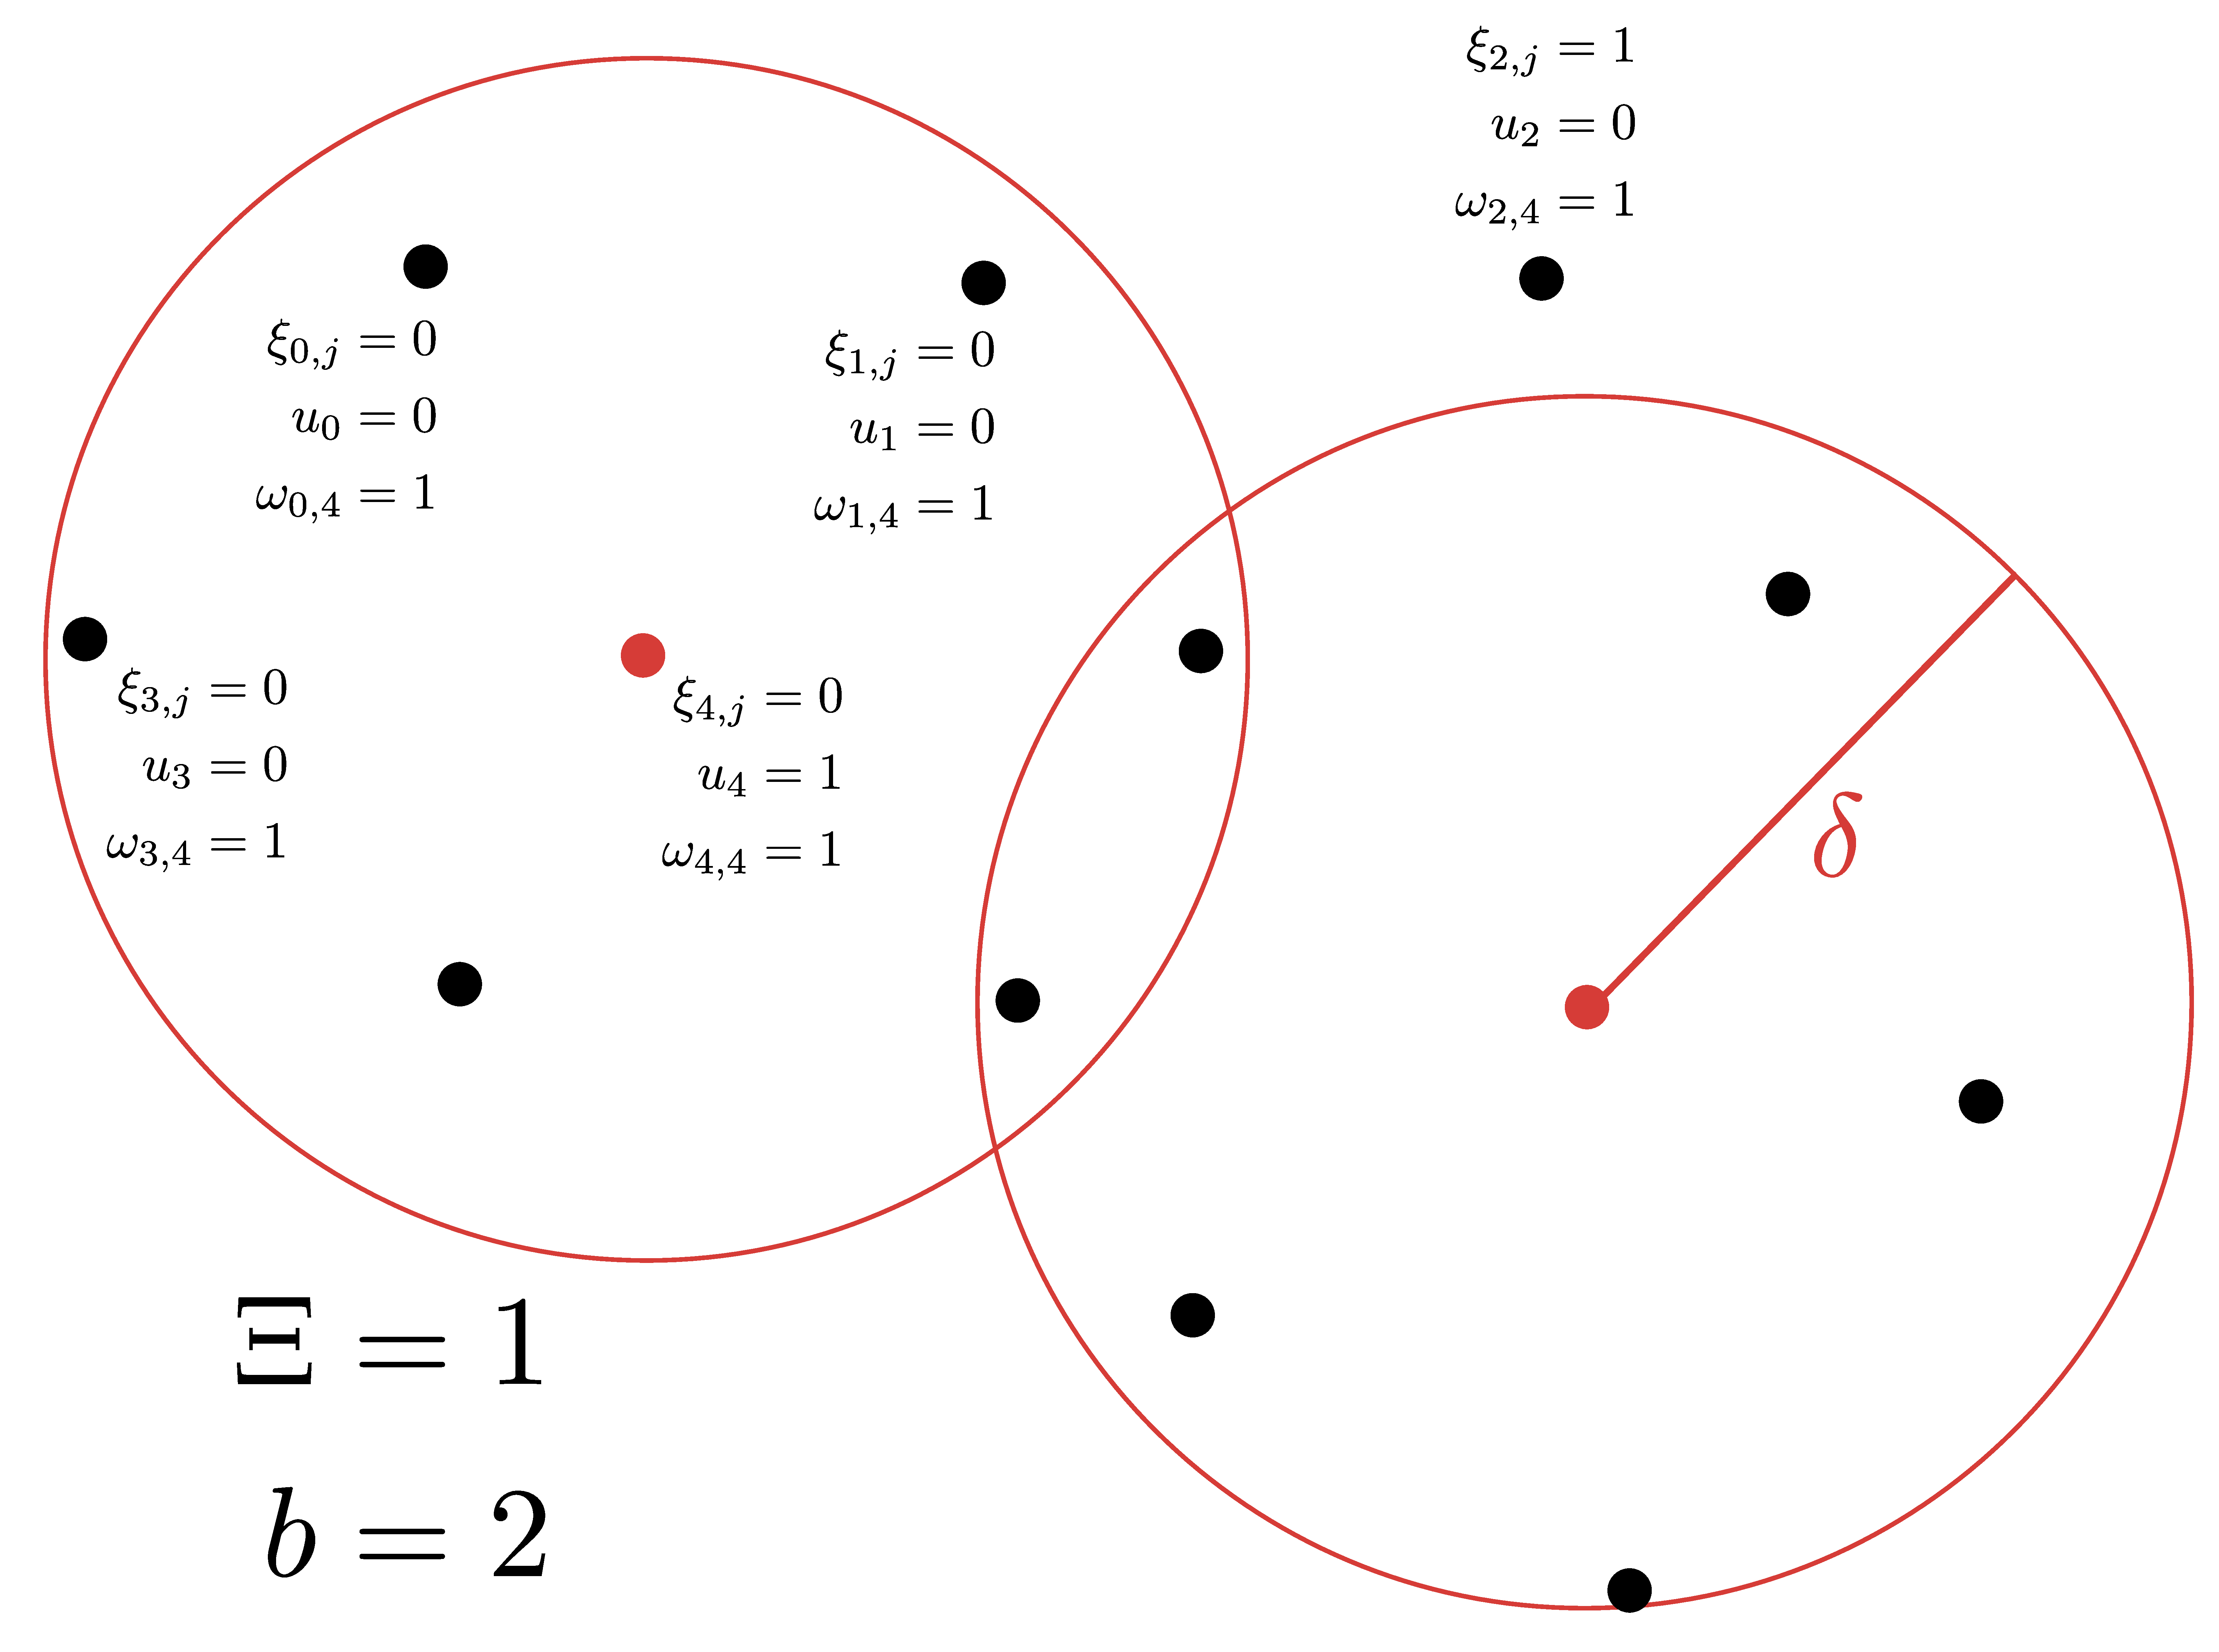
\includegraphics[width=\columnwidth]{mip.pdf}
    \caption{Visualizations of the variables in the mixed integer program. In this solution, $4^{th}$ node is chosen as a center and node $0,1,3$ is ended up in $\delta$ ball around the $4^{th}$ node. The solution also marked $2^{nd}$ node as an outlier by not including it in any $\delta$ ball.}
\label{mip}
\end{figure}


\begin{algorithm}[tb]
   \caption{Robust k-Center}
   \label{alg:bin}
\begin{algorithmic}
   \STATE {\bfseries Input:} data $\mathbf{x}_i$, existing pool $\mathbf{s}^0$, budget $b$ and outlier bound $\Xi$
   \STATE {\bfseries Initialize} $\mathbf{s}_g =$ k-Center-Greedy($\mathbf{x}_i, \mathbf{s}^0, b$)
   \STATE $\delta_{2-OPT} = \max_j \min_{i \in \mathbf{s}_g} \Delta(\mathbf{x}_i,\mathbf{x}_j)$ 
   \STATE $lb=\frac{\delta_{2-OPT}}{2}$, $ub=\delta_{2-OPT}$
   \REPEAT
   \IF {$Feasible(b, \mathbf{s}^0,\frac{lb+ub}{2},\Xi)$}
   \STATE $ub=\max_{i,j \mid  \Delta(\mathbf{x}_i,\mathbf{x}_j) \leq \frac{lb+ub}{2}}  \Delta(\mathbf{x}_i,\mathbf{x}_j) $
   \ELSE
   \STATE $lb=\min_{i,j \mid   \Delta(\mathbf{x}_i,\mathbf{x}_j) \geq \frac{lb+ub}{2}}  \Delta(\mathbf{x}_i,\mathbf{x}_j) $
    \ENDIF
   \UNTIL{$ub = lb$}
      \STATE {\bfseries return} $\{i\ st.\ u_i=1\}$
\end{algorithmic}
\end{algorithm}
\subsection{Implementation Details}
\label{sec:imp}
One of the most important design choices is the distance function $\Delta(\cdot,\cdot)$. We use the $l_2$ distance between activations of the final fully-connected layer as a distance function. For semi-supervised learning, we used Ladder networks\cite{ladder} and for all experiments we used VGG-16\cite{vgg} as a CNN architecture. We optimized all models using RMSProp with learning rate $1\mathrm{e}{-3}$ using Tensorflow\cite{tensorflow}. 

While implementing our algorithm we used Gurobi\cite{gurobi} framework for checking feasibility of the MIP define in (\ref{mipfeasible}). As an upper bound on number of outliers, we used $\Xi=1\mathrm{e}{-4} \times n$ where $n$ is the number of unlabelled data points.

Upon acceptance, we are planning to release the trained models and the source code.

\section{Experimental Results}
\label{sec:exp}
\begin{figure*}[ht]
    \centering
    \begin{subfigure}[b]{0.4927\textwidth}
        
\includegraphics[width=\textwidth]{placeholder1.jpg}
        \caption{Cifar-10}
    \end{subfigure}
    ~ %add desired spacing between images, e. g. ~, \quad, \qquad, \hfill etc. 
    %(or a blank line to force the subfigure onto a new line)
    \begin{subfigure}[b]{0.4927\textwidth}
        
\includegraphics[width=\textwidth]{placeholder1.jpg}
        \caption{Cifar-100}
    \end{subfigure}
    \caption{Results on Active Learning without Semi-Supervision}\label{fig:resnosemi}
%\end{figure*}
%\begin{figure*}[ht]
%    \centering
   \vspace{5mm}

    \begin{subfigure}[b]{0.4927\textwidth}
        
\includegraphics[width=\textwidth]{placeholder1.jpg}
        \caption{Cifar-10}
    \end{subfigure}
    ~ %add desired spacing between images, e. g. ~, \quad, \qquad, \hfill etc. 
    %(or a blank line to force the subfigure onto a new line)
    \begin{subfigure}[b]{0.4927\textwidth}
        
\includegraphics[width=\textwidth]{placeholder1.jpg}
        \caption{Cifar-100}
    \end{subfigure}
    \caption{Results on Active Learning with Semi-Supervision}\label{fig:ressemi}
\end{figure*}

In order to experiment our approach, we tested our algorithm on the problem of image classification. We used the CIFAR\cite{cifar} dataset in our experiments. We choose CIFAR since it is still somewhat challenging and large-scale (50k images).  CIFAR\cite{cifar} dataset is composed of 50k images and each image is labelled with two different labels one coarse-grained and one fine-grained. There are 100 fine-grained categories and there are 10 coarse-grained categories defined as strict super-sets of some of these fine-grained categories. 

We also performed experiment both using semi-supervision and not using semi-supervision. In our experiments, we start with 5k images sampled iid. from the dataset. Semi-supervised algorithm has an access to labelled examples with their labels as well as unlabelled examples without their labels. Fully-supervised algorithm only has an access to the labelled data points. We consider ladder networks\cite{ladder} on VGG16\cite{vgg} as a semi-supervised algorithm and the original VGG16\cite{vgg} as a fully-supervised learning algorithm. We compute the classification accuracy (precision@top-1) as a metric and plot the accuracy vs labelled number of points. At each step, we learned a network from scratch using the provided (queried) data points. We run the query algorithm iteratively; in other words, we solve the discrete optimization problem $\min_{\mathbf{s}^{k+1} : |\mathbf{s}^{k+1}| \leq b} E_{\mathbf{x},y \sim p_\mathcal{Z}} [l(\mathbf{x},y; A_{\mathbf{s}^{0} \cup \ldots, \mathbf{s}^{k+1}})]$ at each iteration for each points on the graph. We present the semi-supervised results in Figure~\ref{fig:ressemi}, and the fully supervised results in Figure~\ref{fig:resnosemi}.

We compare our algorithm with iid. sampling as well as the uncertainty oracle explained in Section~\ref{sec:whatif}. We also compared our algorithm with CEAL \cite{wang2016cost} which is to the-best-of-our-knowledge only active learning algorithm presented for CNNs. Since it is a semi-supervised approach utilizing unlabelled data points, we only include it in semi-supervised analysis.

TALK ABOUT THE RESULTS

\noindent\textbf{Optimality of the k-Center Solution}
Our proposed method is using the greedy 2-OPT solution for k-Center problem as an initialization and checks the feasibility of a mixed integer programming (MIP) program. Internally, we use LP-relaxation of the defined MIP and use branch-and-bound after that. Clearly, MIP does not enjoy a polynomial time solution; hence, the utility obtained by solving this expensive MIP should be investigated. Hence, we compare the average run-time of MIP on a computation node\footnote{some specs} with the run-time of 2-OPT solution in Table~\ref{tab:runtime}. We also compare the accuracy obtained with optimal k-Center solution and the 2-OPT solution in Figure~\ref{fig:twoopt}

\begin{table}[ht]
\centering
\caption{Decomposition of average run-time of our discrete optimization algorithm.}
\begin{tabular}{cccc} \toprule
 & MIP & MIP &  \\
Greedy(2-OPT) & (per iteration) & (total) & Total \\ \midrule
0 sec  & 0 sec & 0 sec & 0 sec \\ \bottomrule
\end{tabular}
\end{table}

As shown in the Table~\ref{tab:runtime}; although the run-time of MIP is not polynomial in worst-case, in practice it converges in a tractable time for dataset of 50k images. It should also be noted that the run time of our algorithm is negligible when compared with query time (asking oracle for labels). Hence, we believe our algorithm can easily be applied to existing deep-learning setups. There are also many approximate and/or distributed solvers for both k-Center and MIP \cite{kcenterdist,gurobi}. Hence, it can also scale to very large datasets of multiple million images.
 
 \begin{figure}[ht]

\includegraphics[width=\columnwidth]{placeholder1.jpg}
\caption{Effect of approximation in set-cover problem.}
\label{fig:twoopt}
\end{figure}

As the Figure~\ref{fig:twoopt} suggests, there is a small, but not negligible, difference between the accuracy when 2-OPT solution is used. Hence, we conclude that unless the scale of the dataset restricts, using our proposed optimal solver is desired. On the other hand, even with the accuracy drop, our active learning strategy using 2-OPT solution still outperforms the other baselines. Hence, we can conclude that our algorithm can scale to any dataset size with small accuracy drop.

\noindent\textbf{Relationship between test error and the space cover.}
Our intuition as well as the theoretical analysis in Section~\ref{sec:analysis} suggests that test error is directly related to the maximum of distance between any unlabelled data point and its nearest labelled neighbor ($\delta$). We further analyze this behavior empirically. We show the scatter plot of test error with respect to the optimization objective $\delta$ in Figure~\ref{fig:scat}.
 
\begin{figure}[ht]

\includegraphics[width=\columnwidth]{placeholder1.jpg}
\caption{Test error vs the maximum of distance between any unlabelled data point and its nearest labelled neighbor($\delta$)}
\label{fig:scat}
\end{figure}

The figure suggest a strong and linear correlation between test error and $\delta$. Hence, we can conclude the bound we present in Theorem~\ref{mainthm2} is very tight in practice and largely explain the behavior.

\section{Analysis of the Algorithm}
\label{sec:analysis}
In this section, we analyze our algorithm in terms of generalization error.  We are typically interested in the error in unseen images $E_{\mathbf{x},y \sim p_\mathcal{Z}}[l(\mathbf{x},y,A_{\mathbf{s}})]$ in terms of the empirical loss over the labelled images $\frac{1}{m}\sum_{j\in[m]} l(\mathbf{x}_{s(i)},y_{s(i)},A_{\mathbf{s}})$. However, this analysis requires joint treatment of the generalization error and the effect of query selection. For simplicity, we divide this analysis into two parts. First, we analyze the relationship between expected loss in unseen images (generalization error) and the empirical loss over the entire dataset ($\frac{1}{n}\sum_{i\in [n]} l(\mathbf{x}_i,y_i,A_\mathbf{s})$). Secondly, we analyze the relationship between the loss over the entire dataset and loss over the labelled samples. We study the first relationship by assuming a Lipschitz continuous loss function. By extending the robustness results from \cite{robust}, we state the following theorem and defer its proof to the supplementary material.

\begin{theorem}
Given $n$ i.i.d. samples drawn from $p_\mathcal{Z}$ as $\{\mathbf{x}_i,y_i\}_{i\in[n]}$. If loss function $l(\cdot,y,\mathbf{w})$ is $\lambda^l$-Lipschitz continuous for all $y, \mathbf{w}$, bounded by $L$ and $\mathcal{X}x\mathcal{Y}$ has a covering number $N_{\epsilon}(\mathcal{X},|\cdot|_2)=K$; with probability at least $(1-\delta)$,
\[
\left|E_{\mathbf{x},y \sim p_\mathcal{Z}}[l(\mathbf{x},y, A_\mathbf{s})] - \frac{1}{n}\sum_{i\in[n]} l(\mathbf{x}_i,y_i,A_\mathbf{s})\right|  \leq  \lambda^l \epsilon + L \sqrt{\frac{2K\log 2 + 2\log (1/\delta)}{n}}
\]
\label{mainthm}
\end{theorem}

First of all, this theorem is applicable to any machine learning algorithm with Lipschitz loss function and we further prove the Lipschitz-continuity of CNNs. It can clearly be seen that the empirical loss converges to the expected loss with large number of data points $n$ since $\lambda^l\epsilon$ term can be made arbitrarily small. In order to complete the study about the generalization performance of CNNs, we prove the Lipschitz-continuity of the loss function of a CNN with the following lemma where max-pool and restricted linear units are the non-linearities and the loss is defined as $l_2$ distance between the desired probabilities and the soft-max outputs.

\begin{lemma}
A convolutional neural network with $n_c$ convolutional (with max-pool and ReLU) and $n_{fc}$ fully connected layers defined over C class with loss function defined as 2-norm between softmax output and class probability is $\left(\frac{\sqrt{C-1}}{C} \alpha^{n_c+n_{fc}}\right)$-Lipschitz.
\end{lemma}

Here, $\alpha$ is the maximum sum of  input weights per neuron (see supplementary materials for formal definition). Although, it is in general unbounded, it can be made arbitrarily small without changing the loss function behavior (\ie keeping the label of any data point $\mathbf{s}$ unchanged). % since dividing all weights with a scalar will not switch any label. Hence, for any CNN, there is an equivalent CNN (in terms of classification function) with $\alpha \leq \varrho$ for any $\varrho > 0$. 
We can conclude that CNNs enjoy a $0$ generalization error in the limiting case thanks to the Lipschitz property.

In order to complete the analysis, we need to study the behavior of the loss over the dataset in terms of the empirical loss over the selected (queried) samples. Here, we make a no training error assumption; in other words, we assume that the training error for labelled images is $0$ at the end of the learning. This is clearly a restrictive assumption, however, it is very feasible due to large parameter space of CNNs. Moreover, this can also be enforced by simply converting average loss into maximal loss via \cite{maximal_loss}. %We did not need this trick since our CNNs reached 0 training error in all experiments. 
Using this assumption, we show that the loss over the entire dataset can be bounded using the result of our discrete optimization problem.% multiplied with a constant factor.

\begin{theorem}
Given $n$ i.i.d. samples drawn from $p_\mathcal{Z}$ as $\{\mathbf{x}_i,y_i\}_{i\in[n]}$, and $m$ chosen points $\{ s(i) \in [N]\}_{\i \in [m]}$. If loss function $l(\cdot,y,\mathbf{w})$ is $\lambda^l$-Lipschitz continuous for all $y, \mathbf{w}$ and bounded by $L$, regression function is $\lambda^\eta$-Lipschitz, $\{ s(i) \in [N]\}_{\i \in [m]}$ is $\delta$ cover of $\{\mathbf{x}_i,y_i\}_{i\in[n]}$, and $l(\mathbf{x}_{s(j)},y_{s(j)},A_\mathbf{S})=0\quad \forall j \in [m]$; with probability at least $1-\gamma$,
\begin{small}
\[
%\frac{1}{n}\sum_i l(\mathbf{x}_i,y_i,A_\mathbf{s}) \leq \mathcal{L}_{[n]} (h^\star) +\delta(\lambda^l + 2 \lambda^{\eta}) + 
%\sqrt{\frac{\log(1/1-\gamma)}{2n}}
\frac{1}{n}\sum_{i \in [n]} l(\mathbf{x}_i,y_i) \leq \delta (\lambda^l + \lambda^\mu LC)+ 
\sqrt{\frac{L \log(1/\gamma)}{2n}}
\]
\end{small}
%where $\mathcal{L}_{[n]} (h^\star)$ is the loss of the Bayes-optimal classifier.
\label{mainthm2}
\end{theorem}

It can easily be shown that in this setting, $\lim_{n \rightarrow \infty} \frac{1}{n}\sum_i l(\mathbf{x}_i,y_i,A_\mathbf{s}) =    \delta (\lambda^l + \lambda^\mu LC)$. Clearly, $\delta$ decreases when $m$ increases; however, the rate is critical. To show that our algorithm have finite query, we need to show that $\delta$ can be made arbitrarily small with finite $m$ in the limiting behavior of number of unlabelled data points (i.e. $n \rightarrow \infty$). Since our data points are coming from a compact space, there exists a finite sub-cover to any union of open sets. Hence, the finite query property is a straightforward result of compactness. %We give the following corollary without proof;

\iffalse
\begin{cor}
Given $n$ i.i.d. samples drawn from $p_\mathcal{Z}$ as $\{\mathbf{x}_i,y_i\}_{i\in[n]}$, and a desired error rate $\rho$. If loss function $l(\cdot,y,\mathbf{w})$ is $\lambda^l$-Lipschitz continuous for all $y, \mathbf{w}$, regression function is $\lambda^\eta$-Lipschitz, there exist a finite subset $\mathbf{s}$ with cardinality m such that any CNN achieving $0$ error over $\{\mathbf{x}_{s(j)},y_{s(j)}\}_{j \in [m]}$ achieve the following with probability $1$.
\[
\lim_{n \rightarrow \infty} \frac{1}{n}\sum_i l(\mathbf{x}_i,y_i) \leq \rho %\mathcal{L}_{[n]} (h^\star) +
\]
%where $\mathcal{L}_{[n]} (h^\star)$ is the loss of the Bayes-optimal classifier.
\label{maincor}
\end{cor}
\fi

In summary, we show that CNNs have Lipschitz continuous loss functions, making them generalize to unseen images. In addition, when the underlying data distribution has Lipschitz continuous regression functions, we further show, under reasonable assumptions, a small subset of dataset is enough to be labelled as long as it covers the space efficiently. Since the difference between the empirical loss over unseen images and the optimal loss is bounded by $\delta(\lambda^l + 2 \lambda^{\eta})$, direct minimization of $\delta$ is a theoretically soundapproach to this problem, validating our space-covering heuristic.


\section{Conclusion}
Suspendisse pharetra erat sapien, sit amet porta mi cursus congue. Sed pulvinar justo in metus sollicitudin mollis. Mauris sagittis dui vitae arcu gravida, et lacinia mauris ultrices. Sed faucibus nibh ac velit vehicula, ac molestie tellus mattis. Duis nec tellus erat. Aliquam pellentesque nibh quis ex blandit euismod porta id leo. In facilisis finibus nisl, rhoncus dignissim dui lobortis sit amet. Nulla pellentesque, nisi ac porta consectetur, lorem nisl rhoncus dolor, sed ornare mi nisi maximus magna. Integer nunc ipsum, lobortis vel diam in, vestibulum iaculis felis. Etiam viverra fermentum scelerisque. Praesent facilisis ultrices magna, sit amet dignissim velit rutrum tempor. Nunc in diam elit. Vestibulum eget molestie erat. 

\clearpage
\bibliography{active_adversarial} 
\bibliographystyle{icml2017}
\end{document} 
